\documentclass[12pt]{article}

\usepackage{amsmath,amsthm,amsfonts,amssymb,amsxtra}
\usepackage{pgf,tikz}
\usetikzlibrary{arrows}
\renewcommand{\theenumi}{(\alph{enumi})} 
\renewcommand{\labelenumi}{\theenumi}

\pagestyle{empty}
\setlength{\textwidth}{7in}
\setlength{\oddsidemargin}{-0.5in}
\setlength{\topmargin}{-1.0in}
\setlength{\textheight}{9.5in}

\theoremstyle{definition}
\newtheorem{problem}{Problem}

\begin{document}

\noindent{\large\bf MATH 242}\hfill{\large\bf Test \#1}\hfill{\large\bf
  Spring 2018}\hfill{\large\bf Page 1/7}\hrule

\bigskip
\begin{center}
  \begin{tabular}{|ll|}
    \hline & \cr
    {\bf Name: } & \makebox[12cm]{\hrulefill}\cr & \cr
    {\bf VIP ID:} & \makebox[12cm]{\hrulefill}\cr & \cr
    \hline
  \end{tabular}
\end{center}
\begin{itemize}
\item Write your name and VIP ID in the space provided above.
\item The test has seven (7) pages, including this one.
\item Enter your answer in the box(es) provided.
\item Show sufficient work to justify all answers unless otherwise
  stated in the problem.  Correct answers with inconsistent work may
  not be given credit. 
\item Credit for each problem is given at the right of each problem
  number. 
\end{itemize}
\hrule

\begin{center}
  \begin{tabular}{|c|c|c|}
    \hline
    &&\cr
    {\large\bf Page} & {\large\bf Max} & {\large\bf Points} \cr
    &&\cr
    \hline
    &&\cr
    {\Large 2} & \Large 20 & \cr
    &&\cr
    \hline
    &&\cr
    {\Large 3} & \Large 10 & \cr
    &&\cr
    \hline
    &&\cr
    {\Large 4} & \Large 20 & \cr
    &&\cr
    \hline
    &&\cr
    {\Large 5} & \Large 20 & \cr
    &&\cr
    \hline
    &&\cr
    {\Large 6} & \Large 20 & \cr
    &&\cr
    \hline
    &&\cr
    {\Large 7} & \Large 10 & \cr
    &&\cr
    \hline\hline
    &&\cr
    {\large\bf Total} & \Large 100 & \cr
    &&\cr
    \hline
  \end{tabular}
\end{center}
\newpage

%%%%%%%%%%%%%%%%%%%%%%%%%%%%%%%%%%%%% Page 2
\noindent{\large\bf MATH 242}\hfill{\large\bf Test \#1}\hfill{\large\bf
  Spring 2018}\hfill{\large\bf Page 2/7}\hrule

  \subsection*{Skills tested on this page:} 
  \begin{center}
  \begin{tabular}{|c|c|c|}
  \hline 
  && \\
  \textbf{Terminology} &
  \textbf{Notation} &
  \textbf{Background Algebra} \\ 
  && \\ \hline
  && \\
  \textbf{Derivatives} &
  \textbf{Integration} &
  \textbf{Management of constants} \\
  && \\ \hline
  \end{tabular}
  \end{center}
  \begin{problem}[20 pts]
  Consider the following \emph{first-order separable} differential equation:
  \begin{equation*}
  y' = x(y+1)
  \end{equation*}
  \begin{enumerate}
    \item \textbf{[5 pts]} Find an \emph{implicit form} of its \textbf{general solution}.
    \vspace{4.25cm}
    \begin{flushright}
    \begin{tikzpicture}
    \draw (0cm,1.4cm) rectangle (7cm,2.8cm);
    \end{tikzpicture}
    \end{flushright}  
    \item \textbf{[5 pts]} Find a \emph{particular solution} that solves the following \textbf{initial value problem}
    \begin{equation*}
    y' = x(y+1), \quad y(0) = e-1
    \end{equation*}
    \begin{flushright}
    \begin{tikzpicture}
    \draw (-0.5cm,2.1cm) node {$y=$};
    \draw (0cm,1.4cm) rectangle (5cm,2.8cm);
    \end{tikzpicture}
    \end{flushright}
    \item \textbf{[5 pts]} Are there any \textbf{singular solutions}?  Find at least one.
    \begin{flushright}
    \begin{tikzpicture}
    \draw (-0.5cm,2.1cm) node {$y=$};
    \draw (0cm,1.4cm) rectangle (5cm,2.8cm);
    \end{tikzpicture}
    \end{flushright}
    \item \textbf{[5 pts]} Find an explicit \emph{particular solution} that solves this other \textbf{initial value problem}
    \begin{equation*}
    y' = x(y+1), \quad y(0) = -1
    \end{equation*}
    \begin{flushright}
    \begin{tikzpicture}
    \draw (-0.5cm,2.1cm) node {$y=$};
    \draw (0cm,1.4cm) rectangle (5cm,2.8cm);
    \end{tikzpicture}
    \end{flushright}
  \end{enumerate}
  \end{problem}
  \newpage

%%%%%%%%%%%%%%%%%%%%%%%%%%%%%%%%%%%%% Page 3
\noindent{\large\bf MATH 242}\hfill{\large\bf Test \#1}\hfill{\large\bf
Spring 2018}\hfill{\large\bf Page 3/7}\hrule

\section*{Skills on this page: Slope fields, Euler's Method}
\begin{problem}[5 pts---all or nothing]
Which of the following is the slope field of the following differential equation?
\begin{equation*}
y' = x^2 -x-2
\end{equation*}
\noindent (You do not need to show work)
\begin{center}
\begin{tabular}{cc}
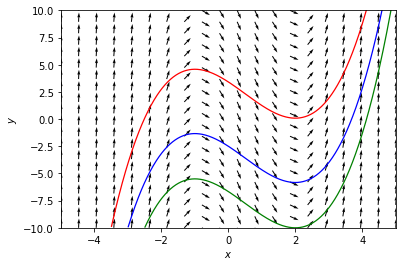
\includegraphics[width=0.5\linewidth]{quiver1.png} &
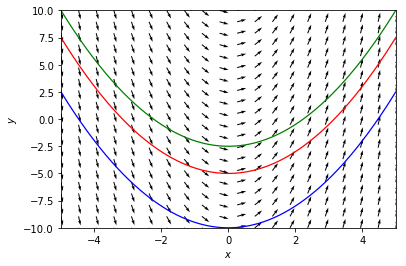
\includegraphics[width=0.5\linewidth]{quiver2.png}
\end{tabular}
\end{center}
\end{problem}
\hrule

\begin{problem}[5 pts]
Use Euler's method with a step size $h=0.5$ to obtain a numerical approximation of the following \textbf{initial value problem}
\begin{equation*}
y' = x^2y, \quad y(0)=1
\end{equation*}
\vspace{5cm}
\begin{flushright}
\begin{tabular}{|c||c|c|c|}
\hline
$n$ & $x_n$ & $y_n$ & $f(x_n, y_n)$ \\ 
\hline \hline
&&& \\
$0$ & \hspace{0.5cm} & \hspace{1cm} & \hspace{3cm} \\
&&& \\ \hline
&&& \\
$1$ &&& \\
&&& \\ \hline
&&& \\
$2$ &&& \\
&&& \\ \hline
\end{tabular}
\end{flushright}
\end{problem}
\newpage


%%%%%%%%%%%%%%%%%%%%%%%%%%%%%%%%%%%%% Page 4
\noindent{\large\bf MATH 242}\hfill{\large\bf Test \#1}\hfill{\large\bf
Spring 2018}\hfill{\large\bf Page 4/7}\hrule

\section*{Skills on this page: First-order differential equations}

\begin{problem}[10 pts]
Solve the following differential equation
\begin{equation*}
\big(e^x+y e^{xy}\big) + \big( e^y+xe^{xy}\big)y' = 0
\end{equation*}

\vspace{6.5cm}
\begin{flushright}
\begin{tikzpicture}
\draw (0cm,-0.2cm) rectangle (7cm,1.2cm);
\end{tikzpicture}
\end{flushright}
\end{problem}
\hrule

\begin{problem}[10 pts]
Solve the following differential equation:
\begin{equation*}
xy' = \sqrt{x^2-y^2} + y
\end{equation*}

\vspace{7.5cm}
\begin{flushright}
\begin{tikzpicture}
\draw (0cm,-0.2cm) rectangle (7cm,1.2cm);
\end{tikzpicture}
\end{flushright}
\end{problem}
\newpage


%%%%%%%%%%%%%%%%%%%%%%%%%%%%%%%%%%%%% Page 4
\noindent{\large\bf MATH 242}\hfill{\large\bf Test \#1}\hfill{\large\bf
Spring 2018}\hfill{\large\bf Page 5/7}\hrule

\section*{Skills on this page: First-order differential equations}

\begin{problem}[20 pts]
Solve the following differential equation:
\begin{equation*}
2x^2y-x^3y'=y^3
\end{equation*}

\vspace{18cm}
\begin{flushright}
\begin{tikzpicture}
\draw (0cm,-0.2cm) rectangle (7cm,1.2cm);
\end{tikzpicture}
\end{flushright}
\end{problem}
\newpage

%%%%%%%%%%%%%%%%%%%%%%%%%%%%%%%%%%%%% Page 4
\noindent{\large\bf MATH 242}\hfill{\large\bf Test \#1}\hfill{\large\bf
Spring 2018}\hfill{\large\bf Page 6/7}\hrule

\section*{Skills on this page: Second-order differential equations}
\begin{problem}[10 pts]
Solve the following initial value problem:
\begin{equation*}
y''+4y=2x-3, \quad y(0)= 1, \quad y'(0)=2
\end{equation*}

\vspace{6cm}
\begin{flushright}
\begin{tikzpicture}
\draw (0cm,-0.2cm) rectangle (7cm,1.2cm);
\end{tikzpicture}
\end{flushright}
\end{problem}
\hrule

\begin{problem}[10 pts]
Solve the following differential equation (assume $y,y'>0$):
\begin{equation*}
y y'' + \big(y'\big)^2=0
\end{equation*}


\vspace{7cm}
\begin{flushright}
\begin{tikzpicture}
\draw (0cm,-0.2cm) rectangle (7cm,1.2cm);
\end{tikzpicture}
\end{flushright}
\end{problem}

\newpage

%%%%%%%%%%%%%%%%%%%%%%%%%%%%%%%%%%%%% Page 4
\noindent{\large\bf MATH 242}\hfill{\large\bf Test \#1}\hfill{\large\bf
Spring 2018}\hfill{\large\bf Page 7/7}\hrule

\section*{Skills on this page: Second-order differential equations}

\begin{problem}[10 pts---5 pts each part]
Given the differential equation $x^2y''-2xy'+2y=0$,
\begin{enumerate}
  \item Verify that the functions $y_1=x$ and $y_2=x^2$ are particular solutions.
  \item Find a particular solution if initial conditions are given by $y(1)=3, y'(1)=1$.

\end{enumerate}
\end{problem}

\end{document}
